\documentclass{beamer}
\usetheme{fibeamer}
\usepackage[utf8]{inputenc}
\usepackage[english]{babel}
\title{Machine Learning with Python} %% that will be typeset on the
\subtitle{Numpy / Matplotlib / Scikit-learn} %% title page.
\author{Luca Erculiani}
%% These additional packages are used within the document:
\usepackage{ragged2e}  % `\justifying` text
\usepackage{booktabs}  % Tables
\usepackage{tabularx}
\usepackage{tikz}      % Diagrams
\usetikzlibrary{calc, shapes, backgrounds}
\usepackage{amsmath, amssymb}
\usepackage{url}       % `\url`s
\usepackage{listings}  % Code listings
\frenchspacing
\begin{document}
  \frame{\maketitle}

\def \bgcc {gray!20!white} 

\defverbatim[colored]\localrun{
\begin{lstlisting}[language=bash,backgroundcolor = \color{\bgcc}]
> ./jupyter-scikit.sh
\end{lstlisting}}
\begin{frame}{Setup}
\framesubtitle{On lab machines}
\centering


\includegraphics[width=0.5\textwidth]{figures/jupyter}

Download and extract the Scikit-learn lecture material from:

{\footnotesize \scriptsize \url{http://disi.unitn.it/~passerini/teaching/2019-2020/MachineLearning/}}

Open the terminal in the folder containing the extracted files and run:
\localrun
%\mint[fontsize=\scriptsize, bgcolor=GGrey]{cucumber}| $> ./jupyter-scikit.sh |

\end{frame}

%-----------------------------------------------------------------------------%

\defverbatim[colored]\pipinstall{
\begin{lstlisting}[language=bash,backgroundcolor = \color{\bgcc}]
> pip install numpy scipy matplotlib sklearn jupyter
\end{lstlisting}}

\defverbatim[colored]\launchjupyter{
\begin{lstlisting}[language=bash,backgroundcolor = \color{\bgcc}]
> jupyter notebook
\end{lstlisting}}

\begin{frame}{Setup}
\framesubtitle{On your own machine}
\centering

Make sure you are using Python 3 for the following steps.

\vspace{0.1in}

Install Numpy, Scipy, Matplotlib, Scikit-learn and Jupyter:
\pipinstall
%\mint[fontsize=\scriptsize, bgcolor=GGrey]{cucumber}| $> pip install numpy scipy matplotlib sklearn jupyter |

\vspace{0.2in}

Download and extract the material for the Scikit-learn lab:


{\footnotesize \scriptsize \url{http://disi.unitn.it/~passerini/teaching/2019-2020/MachineLearning/}}

Open the terminal in the folder containing the extracted files and run:
\launchjupyter
%\mint[fontsize=\scriptsize, bgcolor=GGrey]{cucumber}| $> jupyter notebook |

\end{frame}

%-----------------------------------------------------------------------------%

\begin{frame}{Setup}
\framesubtitle{Jupyter notebook}
\centering

Open the browser at the given address and you'll see something like:

\vspace{0.2in}
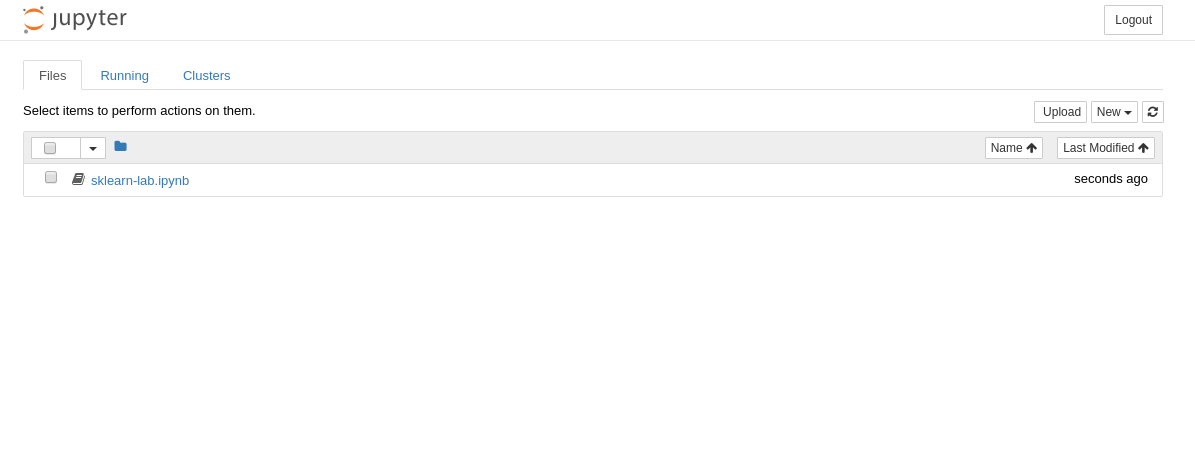
\includegraphics[width=\textwidth]{figures/home}

\vspace{-0.8in}

Open the \texttt{sklearn-lab.ipynb} file containing the lecture notebook.

\end{frame}

%-----------------------------------------------------------------------------%

\begin{frame}{Jupyter notebook}
\centering

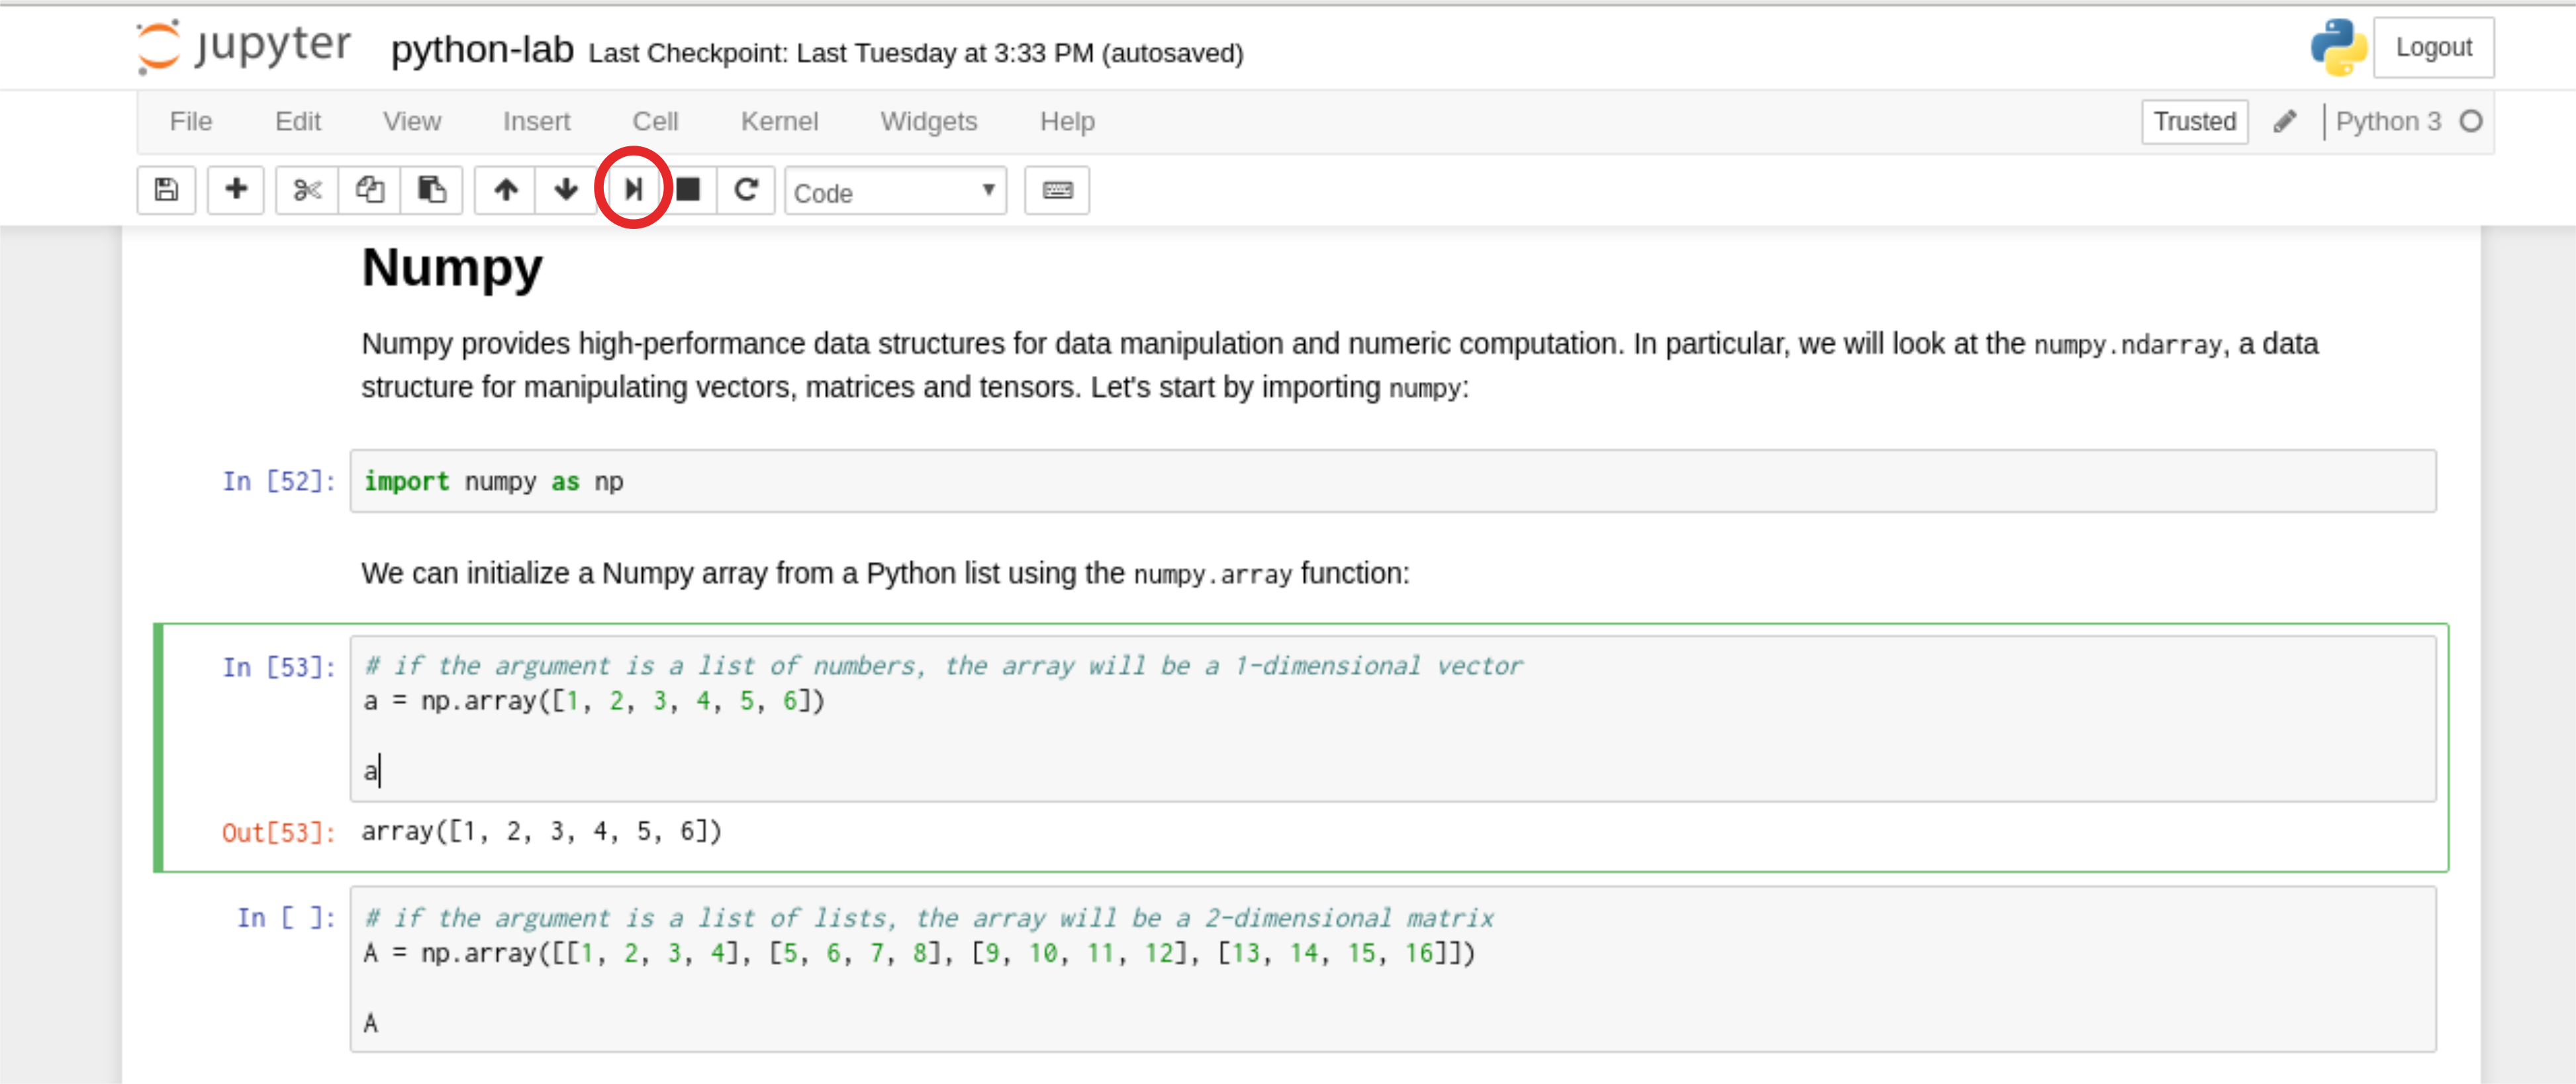
\includegraphics[width=\textwidth]{figures/click1}

\vspace{0.1in}
\hrule
\vspace{0.1in}

Execute commands by selecting a cell and clicking the \textcolor{red}{Run
button} on the header of the page or by \textbf{Shift+Enter}. You will see the
output of the command just below the cell.

You can tweak and modify the code as you wish and execute it again.

\end{frame}

%-----------------------------------------------------------------------------%

\begin{frame}{Assignment}
\centering

For the second Machine Learning assignment you will solve a classification task
using \textbf{Scikit-learn} over some given dataset. Each available dataset is
already split into training and test sets. Your task is to
choose a dataset, train a classifier on the training set and predict the labels
on the test set. To pass the assignment, your classifier has to classify the
examples in the test set with higher accuracy than the reference baseline for
the chosen dataset.

Additionally, you need to test your algorithm via cross-validation over the
training set and produce a report containing the results obtained.

\end{frame}

%-----------------------------------------------------------------------------%

\begin{frame}{Assignment}
\framesubtitle{Datasets}
\centering

\vspace{0.1in}

{\def\arraystretch{2}\tabcolsep=10pt
\begin{tabular}{cc}
    \centering
    \shortstack{\textbf{OCR} \\ Optical Character Recognition} & \shortstack{\textbf{Spambase} \\ Spam email classification} \\
    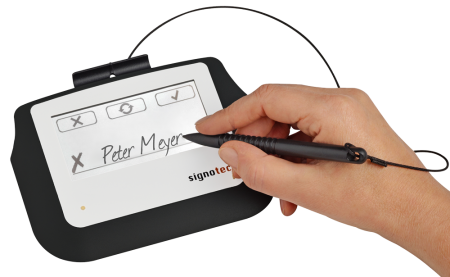
\includegraphics[height=0.2\textheight]{figures/signature} & 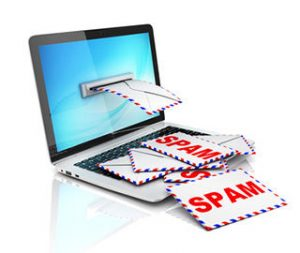
\includegraphics[height=0.2\textheight]{figures/spam} \\
    
    \multicolumn{2}{c}{\shortstack{\textbf{Presidential campaign tweets} \\ Classification of tweets from D. Trump and H. Clinton}} \\
    \multicolumn{2}{c}{
\includegraphics[width=0.5\textwidth]{figures/tweet}} \\
\end{tabular}
}

\end{frame}

%-----------------------------------------------------------------------------%

\begin{frame}{Assignment}
\framesubtitle{Material}
Download the assignment material:

{\scriptsize \url{http://disi.unitn.it/~passerini/teaching/2019-2020/MachineLearning/}}

The material contains the three datasets, each one containing:
    \begin{itemize}
    \item The training set examples;
    \item The training set labels;
    \item The test set examples;
    \item The test set labels;
    \item A README containing info about the dataset. \\ this file also contains
          the reference baseline accuracy;
    \item Other info files.
    \end{itemize}

\end{frame}

%-----------------------------------------------------------------------------%

%\begin{frame}{Assignment | Helper}
%
%The helper script can be used to test your predictions. Given a file containing
%the predicted labels, the helper script sends the labels to our server and
%receives the prediction accuracy. You can use it in this way:
%
%\mint[fontsize=\scriptsize, bgcolor=GGrey]{cucumber}| >> ./helper.py your.email dataset test-labels.txt |
%
%\vspace{-0.3in}
%The first parameter is your \texttt{unitn} email, the second parameter is the
%dataset label (one among ``ocr'', ``spambase'' and ``tweets''), the third
%parameter is the path to the file containing the predicted labels. This file
%should contain one label per line in the same order of the file containing the
%examples. The labels should be in the same format of the labels in the training
%set.
%
%The helper also prints the current best accuracy achieved by any of you on that
%dataset, just to put a bit of healthy competition! :)
%
%\end{frame}

%-----------------------------------------------------------------------------%

\begin{frame}{Assignment}
\framesubtitle{Step-by-step}

\begin{enumerate}
\item Choose a dataset;
\item Experiment with a classification algorithm of your choosing;
\item Test your classifier using cross-validation over the training set
\item Train your classifier over the full training set;
\item Use the classifier to predict the examples in the test set;
\item Place the labels in a file, in the same order as you read the test
      examples and in the same format of the labels in the training set.
\end{enumerate}

\end{frame}

\begin{frame}{Assignment}
\framesubtitle{Report}

Write a report describing the learning algorithm used and discussing the
results obtained; The report should contain at least:
    \begin{itemize}
    \item The average precision, recall, and $F_1$ over the cross validation folds
	    and over the test set. \\ Using
          \texttt{cross\_val\_score} you can specify \texttt{'precision'},
          \texttt{'recall'} and \texttt{'f1'} for the \texttt{scoring}
          parameter. \\ For the OCR dataset, in which you do multiclass
          classification, use weighted averaging, i.e. using
          \texttt{'precision\_weighted'}, \texttt{'recall\_weighted'} and
          \texttt{'f1\_weighted'}; 
    \item The plot of the learning curve, as shown in the lecture;
    \end{itemize}

\end{frame}
%-----------------------------------------------------------------------------%

\begin{frame}{Assignment}
\framesubtitle{Submit}

\begin{itemize}
    \item After completing the assignment submit it via email
    \item Send an email to \href{mailto:mllab@unitn.it}{mllab@unitn.it} 
    \item Subject: sklearnSubmit2019
    \item Attachment: \texttt{id\_name\_surname.zip} containing:
    \begin{itemize}
	    \item The text file, named \texttt{test-pred.txt},  containing the final predictions;
        \item The code used to produce the predictions, the results and the plots;
        \item The report in PDF format.
    \end{itemize}
\end{itemize}
\begin{alertblock}{NOTE}
    \begin{itemize}
	\item \textbf{No group work}
        \item This assignment is mandatory in order to enroll to the oral exam
    \end{itemize}
\end{alertblock}

\end{frame}

\end{document}
